\chapter{Magic}
\section{Which one did you change?}
\section{What day of the month is your birthday?}
It is simple but this 'trick' shows the principles of binary and the power of algorithms.I wish I had invented this one.

1.	Say to the participant "If you answer 5 simple questions I can predict which number in the month your birthday is on"

2.	Question 1 "Is the number in Box A?" If the number is the box add 1 otherwise don't add anything. The Magician keeps a running total of the scores.
\begin{figure}
    \centering
    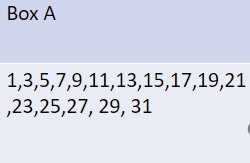
\includegraphics[width=3cm]{chapters/chapterCT1/boxA.png}
    \caption{Box A}
    \label{fig:Box A}
\end{figure}
3.	Question 2 “Is the number in Box B?" If the number is the box add 2 otherwise don't add anything
\begin{figure}
    \centering
    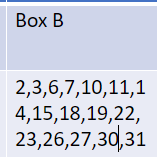
\includegraphics[width=3cm]{chapters/chapterCT1/BoxB.png}
    \caption{Box B}
    \label{fig:Box B}
\end{figure}
4.	Question 3 “Is the number in Box C?" If the number is the box add 4 otherwise don't add anything
\begin{figure}
    \centering
    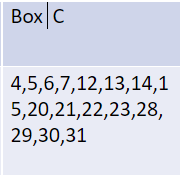
\includegraphics[width=3cm]{chapters/chapterCT1/BoxC.png}
    \caption{Box C}
    \label{fig:Box C}
\end{figure}
5.	Question 4 “Is the number in Box D?" If the number is the box add 8 otherwise don't add anything.
\begin{figure}
    \centering
    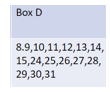
\includegraphics[width=3cm]{chapters/chapterCT1/figures/boxD.png}
    \caption{Box D}
    \label{fig:Box D}
\end{figure}
6.	Question 5 “Is the number in Box E?" If the number is the box add 16 otherwise don't add anything.
\begin{figure}
    \centering
    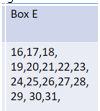
\includegraphics[width=3cm]{chapters/chapterCT1/figures/BoxE.png}
    \caption{Box E}
    \label{fig:Box E}
\end{figure}
7.	Your running total should be the number
What have you done: You have used binary to find the number. For example 27 would be in Box E, Box D , Box B and Box A.which in if we replace the boxes with 1 if the number is in there and 0 if it isn’t; when the boxes are ordered E D C B A we get 11011 which is 27 in decimals. We also have used an algorithm instructions 1 to 6 to get there.
\newline
So lets make it a bit more 'Computer Sciencey,'
Now if we place them into a Table 
\begin{tabular}{lllll} \hline
E & D & C & B & A	 	 \\ \hline
1  & 1  & 0 &  1 & 1\\ \hline

\end{tabular}

Lets instead of A to E we replace the labels with 1, 2,4. 8, 16 each one is the double of the earlier we get:


So 27 is 11011 in binary
\begin{tabular}{lllll} \hline
32 & 16 & 8 & 2 & 1 	 \\ \hline
1  & 1  & 0 &  1 & 1\\ \hline

\end{tabular}

\section{Sorting out VIPS}